\documentclass{article}

\usepackage[utf8]{inputenc}
\usepackage{amsthm}
\usepackage{amssymb}
\usepackage{mathtools}
\usepackage{graphicx}
\usepackage{mdframed}
\usepackage{float}
\usepackage[top=1in, bottom=1.25in, left=1.25in, right=1.25in]{geometry}

\DeclarePairedDelimiter{\abs}{\lvert}{\rvert}
\DeclarePairedDelimiter{\norm}{\lvert \lvert}{\rvert \rvert}

\newtheoremstyle{break}% name
  {}%         Space above, empty = `usual value'
  {}%         Space below
  {\itshape}% Body font
  {}%         Indent amount (empty = no indent, \parindent = para indent)
  {\bfseries}% Thm head font
  {.}%        Punctuation after thm head
  {\newline}% Space after thm head: \newline = linebreak
  {}%         Thm head spec

\newtheorem{Def}{Definition}[section]

\theoremstyle{break}

\newtheorem{innerEx}{Exempel}[section]
\newtheorem{sats}{Sats}[section]
\newtheorem{Rem}{Anmärkning}[section]

\newenvironment{Ex}
{\begin{mdframed} \begin{innerEx} \vspace{3pt}}
{\vspace{3pt} \end{innerEx} \end{mdframed}}  

\newenvironment{bevis}
{\begin{mdframed} \begin{proof} \vspace{3pt}}
{\vspace{3pt} \end{proof} \end{mdframed}}

\title{
    Linjär Algebra\\
    Föreläsning 3
    \author{Erik Sjöström}
}

\begin{document}

\maketitle

\section{Mer om kryssprodukten} % (fold)
\label{sec:mer_om_kryssprodukten}

Det gäller också att:
\begin{equation}
    \norm{\vec{u} \times \vec{v}} = \norm{\vec{u}} \cdot \norm{\vec{v}} \cdot \sin{\alpha}
\end{equation}
\begin{center}
    \vspace{3pt}
    \centering
    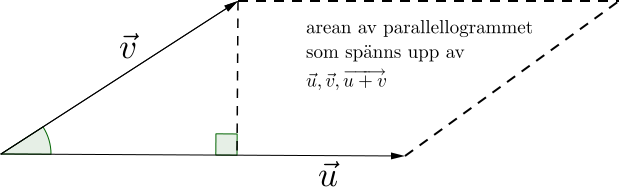
\includegraphics[scale=0.5]{areakryss.png}
\end{center}
\begin{Ex}
    Beräkna arean av triangeln med hörn i:
    \[
        A = (1,1,0),\mbox{ } B = (3,0,2),\mbox{ } C = (0,-1,1) 
    \]
    \begin{center}
        \centering 
        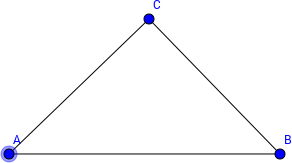
\includegraphics[scale=0.5]{triangle.png}
    \end{center}
    Lösning:
    \begin{align*}
        \frac{1}{2} \norm{\overrightarrow{AB} \times \overrightarrow{AC}} = \frac{1}{2}\norm{\begin{bmatrix} 3-1\\0-1\\2-0 \end{bmatrix} \times \begin{bmatrix} 0-1\\-1-1\\1-0 \end{bmatrix}} = \frac{1}{2} \norm{\begin{bmatrix} 3\\-4\\-5 \end{bmatrix}} = \frac{1}{2}\sqrt{9+16+25} = \frac{5}{\sqrt{2}}
    \end{align*}
\end{Ex}
% section mer_om_kryssprodukten (end)
\newpage
\section{Linjer och plan} % (fold)
\label{sec:linjer_och_plan}
För att beskriva en linje i $\mathbb{R}^2$ behövs en skärning med y-axeln (m) och lutningen (k).
\begin{align}
    &y = k \cdot x + m &&\mbox{Linjens ekvation}
\end{align}
För att beskriva ett plan i $\mathbb{R}^3$ behövs en punkt $p_0 = \begin{bmatrix} x_0&y_0&z_0 \end{bmatrix}$ i planet och en vektor $\vec{n} = \begin{bmatrix} A &B &C \end{bmatrix}$, ortogonal mot planet.\\
Varje annan punkt $Q = \begin{bmatrix} x &y &z \end{bmatrix}$ ligger i planet om vektorn $\overrightarrow{P_0Q} \perp \vec{n}$. Dvs att:
\[
    \overrightarrow{P_0Q} \cdot \vec{n} = 0
\]
Eftersom:
\[
    \overrightarrow{P_0Q} = \begin{bmatrix} x-x_0\\y-y_0\\z-z_0 \end{bmatrix}
\]
får vi att:
\begin{align*}
0 = \overrightarrow{P_0Q} \cdot \vec{n} &= \begin{bmatrix} x-x_0 &y-y_0 &z-z_0 \end{bmatrix} \begin{bmatrix} A\\B\\C \end{bmatrix} \\&= A(x-x_0) + B(y-y_0) + C(z-z_0) \\&= Ax + By + Cz - Ax_0 - By_0 - Cz_0 = 0
\end{align*}
Vi ersätter $(Ax_0 - By_0 - Cz_0)$ med en konstant $D$, och får då:
\[
    Ax + By + Cz = D
\]
Vilket är planets ekvation på normalform. Med normalvektorn $\vec{n} = \begin{bmatrix} A\\B\\C \end{bmatrix}$
\begin{center}
    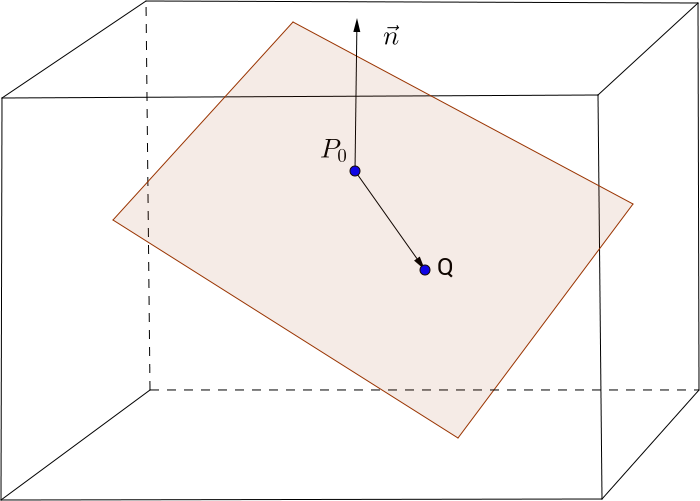
\includegraphics[scale=0.3]{planet.png}
\end{center}
\newpage
\begin{Ex}
    Bestäm planet på normalform, givet:
    \[
        P_0 = \begin{bmatrix} 3\\-1\\7 \end{bmatrix} \mbox{ och } \vec{n} = \begin{bmatrix} 4\\2\\-5 \end{bmatrix}
    \]
    Lösning: Vi får:
    \begin{align*}
    A(x-x_0) + B(y-y_0) + C(z-z_0) &= 4(x-3) + 2(y+1) -5(z-7)\\&= 4x + 2y -5z + 25 = 0
    \end{align*}
\end{Ex}
\begin{Ex}
    Bestäm planets ekvation på normalform för planet mellan punkterna:
    \[
        p_1 = \begin{bmatrix} 1\\2\\-1 \end{bmatrix}, p_2 = \begin{bmatrix} 2\\3\\1 \end{bmatrix}, p_3 = \begin{bmatrix} 3\\-1\\2 \end{bmatrix}
    \]
    \begin{center}
        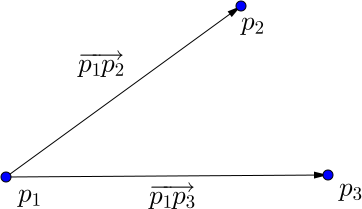
\includegraphics[scale=0.4]{exempel.png}
    \end{center}
    Lösning: Eftersom $p_1, p_2, p_3$ ligger i planet är:
    \[
        \overrightarrow{p_1p_2} = \begin{bmatrix} 2-1\\3-2\\1+1 \end{bmatrix} = \begin{bmatrix} 1\\1\\2 \end{bmatrix} \mbox{ , } \overrightarrow{p_1p_3} = \begin{bmatrix} 2\\-3\\3 \end{bmatrix}
    \]
    parallella med planet.\\
    Och:
    \[
        \vec{n} = \overrightarrow{p_1p_2} \times \overrightarrow{p_1p_3} = \begin{bmatrix} 9\\1\\-5 \end{bmatrix}
    \]
    är ortogonal mot planet. Och alltså en normalvektor.\\
    Dvs: Vi får
    \[
        9(x-1) + y -5z - 16 = 0
    \]
\end{Ex}
\newpage
\noindent
Ett plan kan också ges av en punkt $P_0$ och två vektorer $\vec{u} = \begin{bmatrix} u_1u_2u_3 \end{bmatrix}$ och $\vec{v} = \begin{bmatrix} v_1v_2v_3 \end{bmatrix}$ i planet.\\
Planet består av alla punkter $P$ så att:
\begin{align*}
&P = P_0 + s \cdot \vec{u} + t \cdot \vec{v}\mbox{  } &&s,t \in \mathbb{R}
\end{align*}
\begin{Ex}
    \[
        P_0 = \begin{bmatrix} 1\\2\\3 \end{bmatrix}, \vec{u} = \begin{bmatrix} -1\\2\\2 \end{bmatrix}, \vec{v} = \begin{bmatrix} 2\\1\\5 \end{bmatrix}
    \]
    \[
        P = \begin{bmatrix} x\\y\\z \end{bmatrix} = \begin{bmatrix} 1\\2\\3 \end{bmatrix} + s \begin{bmatrix} -1\\2\\2 \end{bmatrix} + t \begin{bmatrix} 2\\1\\5 \end{bmatrix}
    \]
    eller på parameterform:
    \[
        \begin{cases}
            x = 1-s + 2t \\
            y = 2+2s +t \\
            z = 3+2s +5t
        \end{cases}
    \]
    Byt representation till normalform genom att bestämma $\vec{n} = \vec{u} \times \vec{v}$:
    \[
        \vec{u} \times \vec{v} = \begin{bmatrix} 8\\9\\-5 \end{bmatrix} 
    \]
    Och planet:
    \begin{align*}
    8(x-1) + 9(y-2) - 5(z-3) = 8x + 9y - 5z = 11
    \end{align*}
\end{Ex}
% section linjer_och_plan (end)
\section{Linjer i $\mathbb{R}^3$} % (fold)
\label{sec:linjer_i_}
Antag att att Linjen $L$ är parallell med vektorn $\vec{v} = \begin{bmatrix} v_1&v_2&v_3 \end{bmatrix}$ och går igenom punkten $P_0 = \begin{bmatrix} x_0&y_0&z_0 \end{bmatrix}$
\begin{center}
    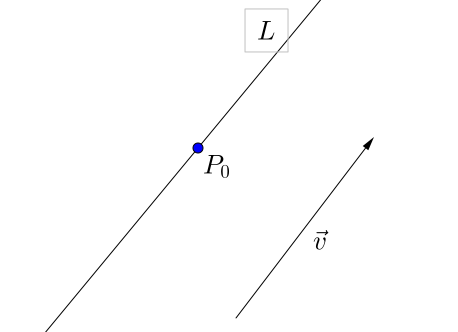
\includegraphics[scale=0.4]{lineandvector.png}
\end{center}
L består av alla punkter P = $\begin{bmatrix} x&y&z \end{bmatrix}$ sådana att $\overrightarrow{P_0P}$ är parallell med $\vec{v}$. \\
\newpage
\noindent
Dvs:
\begin{align*}
&\overrightarrow{P_0P} = t \cdot \vec{v} &&t\in \mathbb{R}
\end{align*}
Eller:
\begin{align*}
&\begin{bmatrix} x-x_0\\y-y_0\\z-z_0 \end{bmatrix} = t \cdot \begin{bmatrix} v_1\\v_2\\v_3 \end{bmatrix} &\begin{cases} x = x_0 + tv_1\\y=y_0+tv_2\\z=z_0tv_3 \end{cases}
\end{align*}
\begin{Ex}
    Linjen genom punkten $\begin{bmatrix} 1&2&-3 \end{bmatrix}$ parallell med \\ $\vec{v} = \begin{bmatrix} 5&5&-7 \end{bmatrix}$ kan parameterframställas som:
    \begin{align*}
    &\begin{cases}
        x=1+4t\\y=2+5t\\z=-3-7t
    \end{cases}
    &&t\in \mathbb{R}
    \end{align*}
    Lös ut t:
    \begin{align*}
    &t=\frac{x-1}{4}, &&t=\frac{y-2}{5}, &&&t=\frac{z+3}{-7}
    \end{align*}
    Vi får:
    \[
        \frac{x-x_0}{v_1} = \frac{y-y_0}{v_2} = \frac{z-z_0}{-7}
    \]
\end{Ex}
\begin{Ex} (a)\\
    Bestäm en ekvation för linjen $L$ som går genom punkterna:
    \[
        P_1 = \begin{bmatrix} 2\\4\\-1 \end{bmatrix}, P_2 = \begin{bmatrix} 5\\0\\7 \end{bmatrix}
    \]
    \begin{center}
        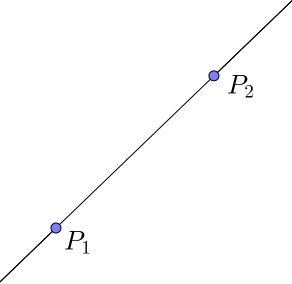
\includegraphics[scale=0.3]{line.png}
    \end{center}
    Lösning:
    Eftersom $\overrightarrow{P_1P_2} = \begin{bmatrix} 3\\-4\\8 \end{bmatrix}$ är parallell med L, och $P_1$ ligger på L ges linjen av:
    \begin{align*}
    &\begin{cases}
        x=2+3t\\y=4-4t\\z=-1+8t
    \end{cases}
    &&t\in \mathbb{R}
    \end{align*}
\end{Ex}
\newpage
\begin{Ex} (b)\\
    I vilken punkt skär linjen från exemplet ovan xy-planet?
    \begin{center}
        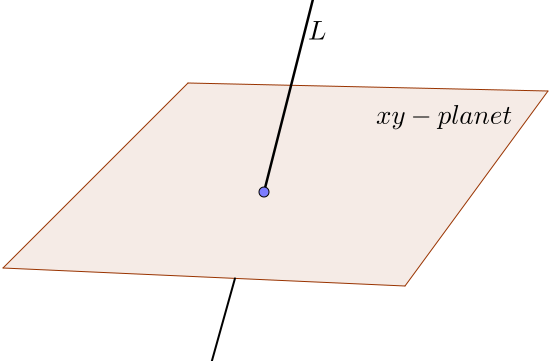
\includegraphics[scale=0.5]{linjeskarplan.png}
    \end{center}
    Sätt $z = 0$:
    \[
        0 = -1 + 8t \Leftrightarrow t = \frac{1}{8}
    \]
    Vi får:
    \begin{align*}
    &x= 2 + 3 \frac{1}{8} = \frac{19}{8}
    &y=4-4 \frac{1}{8} = \frac{7}{2}
    \end{align*}
    Svar: Den skär i punkten:
    \[
        \begin{bmatrix} \frac{19}{8} & \frac{7}{2} & 0 \end{bmatrix}
    \]
    
\end{Ex}



% section linjer_i_ (end)
\end{document} 






















